\documentclass[a4paper,11pt]{article}

%%%%%%%%%%%%%%%%%%%%%%%%%%%%%%%%%%%%%%%%%%%%%%%%%%%%%%%%%%%%%%%%%%%%%%%%
% Paquetes utilizados
%%%%%%%%%%%%%%%%%%%%%%%%%%%%%%%%%%%%%%%%%%%%%%%%%%%%%%%%%%%%%%%%%%%%%%%%

% Gráficos complejos
\usepackage{graphicx}
\usepackage{caption}
\usepackage{subcaption}
\usepackage{placeins}

% Soporte para el lenguaje español
\usepackage{textcomp}
\usepackage[utf8]{inputenc}
\usepackage[T1]{fontenc}
\DeclareUnicodeCharacter{B0}{\textdegree}
\usepackage[spanish]{babel}

% Código fuente embebido
\usepackage{listings}
\usepackage{courier}

% PDFs embebidos para el apéndice
\usepackage{pdfpages}

% Matemáticos
\usepackage{amssymb,amsmath}

% Tablas complejas
\usepackage{multirow}

% Formato de párrafo
\setlength{\parskip}{1ex plus 0.5ex minus 0.2ex}

% Formato de listados de código
\lstset{
  basicstyle=\footnotesize\ttfamily,
  numbers=left,
  numberstyle=\tiny,
  numbersep=5pt,
  tabsize=2,
  extendedchars=true,
  breaklines=true,
  frame=t,
  showspaces=false,
  showtabs=false,
  showstringspaces=false,
  language=Java,
  caption=\lstname,
  captionpos=t
}

%%%%%%%%%%%%%%%%%%%%%%%%%%%%%%%%%%%%%%%%%%%%%%%%%%%%%%%%%%%%%%%%%%%%%%%%
% Título
%%%%%%%%%%%%%%%%%%%%%%%%%%%%%%%%%%%%%%%%%%%%%%%%%%%%%%%%%%%%%%%%%%%%%%%%

% Título principal del documento.
\title{\textbf{Trabajo Práctico N°2}}

% Información sobre los autores.
\author{
  Andrés Gastón Arana(and2arana@gmail.com), \textit{P. 86.203}     \\
  Gabriel Ostrowsky(gaby.ostro@gmail.com), \textit{P. 90762}       \\
  Ignacio Garay Ojeda(imgarayojeda@gmail.com), \textit{P. 92265}   \\
  Pablo Angelini(pablo.angelini@gmail.com), \textit{P. 92265}      \\
  \normalsize{1er. Cuatrimestre de 2013}                           \\
  \normalsize{75.10 - Técnicas de Diseño}                          \\
  \normalsize{Facultad de Ingeniería, Universidad de Buenos Aires}
}
\date{}

%%%%%%%%%%%%%%%%%%%%%%%%%%%%%%%%%%%%%%%%%%%%%%%%%%%%%%%%%%%%%%%%%%%%%%%%
% Documento
%%%%%%%%%%%%%%%%%%%%%%%%%%%%%%%%%%%%%%%%%%%%%%%%%%%%%%%%%%%%%%%%%%%%%%%%

\begin{document}

% ----------------------------------------------------------------------
% Top matter
% ----------------------------------------------------------------------
\thispagestyle{empty}
\maketitle

\begin{abstract}

  Este informe sumariza el desarrollo del trabajo práctico grupal N°2 de la
  materia Técnicas de Diseño (75.10) dictada en el primer cuatrimestre de 2013
  en la Facultad de Ingeniería de la Universidad de Buenos Aires. El mismo
  consiste en el desarrollo de una aplicación de consola minimalista para
  soportar las operaciones de una caja de una cadena de supermercados, 
  aplicando los descuentos correspondientes vigentes al momento de la compra.

\end{abstract}

\clearpage

% ----------------------------------------------------------------------
% Tabla de contenidos
% ----------------------------------------------------------------------
\tableofcontents
\clearpage


% ----------------------------------------------------------------------
% Desarrollo
% ----------------------------------------------------------------------
\part{Desarrollo}
En esta sección se detallan algunas de las decisiones de diseño tomadas. Las 
mismas tienen en cuenta la forma de proveer los Productos y Ofertas disponibles, 
asi como también la implementación de las Ofertas Globales y Exclusivas.

A continuación se muestran los diagramas creados explicando el modelo de la aplicación.

% Inclusión de una imagen - CONFIGURAR PATH!
\begin{figure}[!htp]
\begin{center}
\includegraphics[width=1\textwidth]{./diagramaClases.png}
\end{center}
\caption{Diagrama de Clases} \label{fig001}
\end{figure}

\subsection{Carga de Productos y Ofertas}



\subsection{Condición de Ofertas Exclusivas}
Existe un supuesto a la asignación de ofertas exclusivas para los productos. 
Estas ofertas, como es sabido, no pueden tener multiple asignación a un mismo producto. 
Es decir, cada producto puede tener como máximo una única oferta exclusiva asignada. 
De esta forma, las ofertas son evaluadas por items listados en la compra. De modo que si un item 
con determinada cantidad del mismo producto, llegara a aplicar para una oferta exclusiva, 
ya sea con la cantidad total del item o menor, el item completo quedará marcado como 
"\textit{DescuentoAplicado}" más allá de que sobre alguna cantidad de productos los cuales exceden
los requisitos de la oferta.
Por esto, si un descuento es aplicado a un item, este quedará descartado para ser evaluado 
en el resto de las ofertas exclusivas.

Efectivamente, nuestro algoritmo de selección de las ofertas exclusivas para los productos 
es asignar la primer oferta que cumple con todos los requisitos.

\clearpage

\part{Apéndice}
\appendix

\section{Código fuente}

\FloatBarrier
\clearpage

\section{Enunciado original}\label{sec:enunciado}
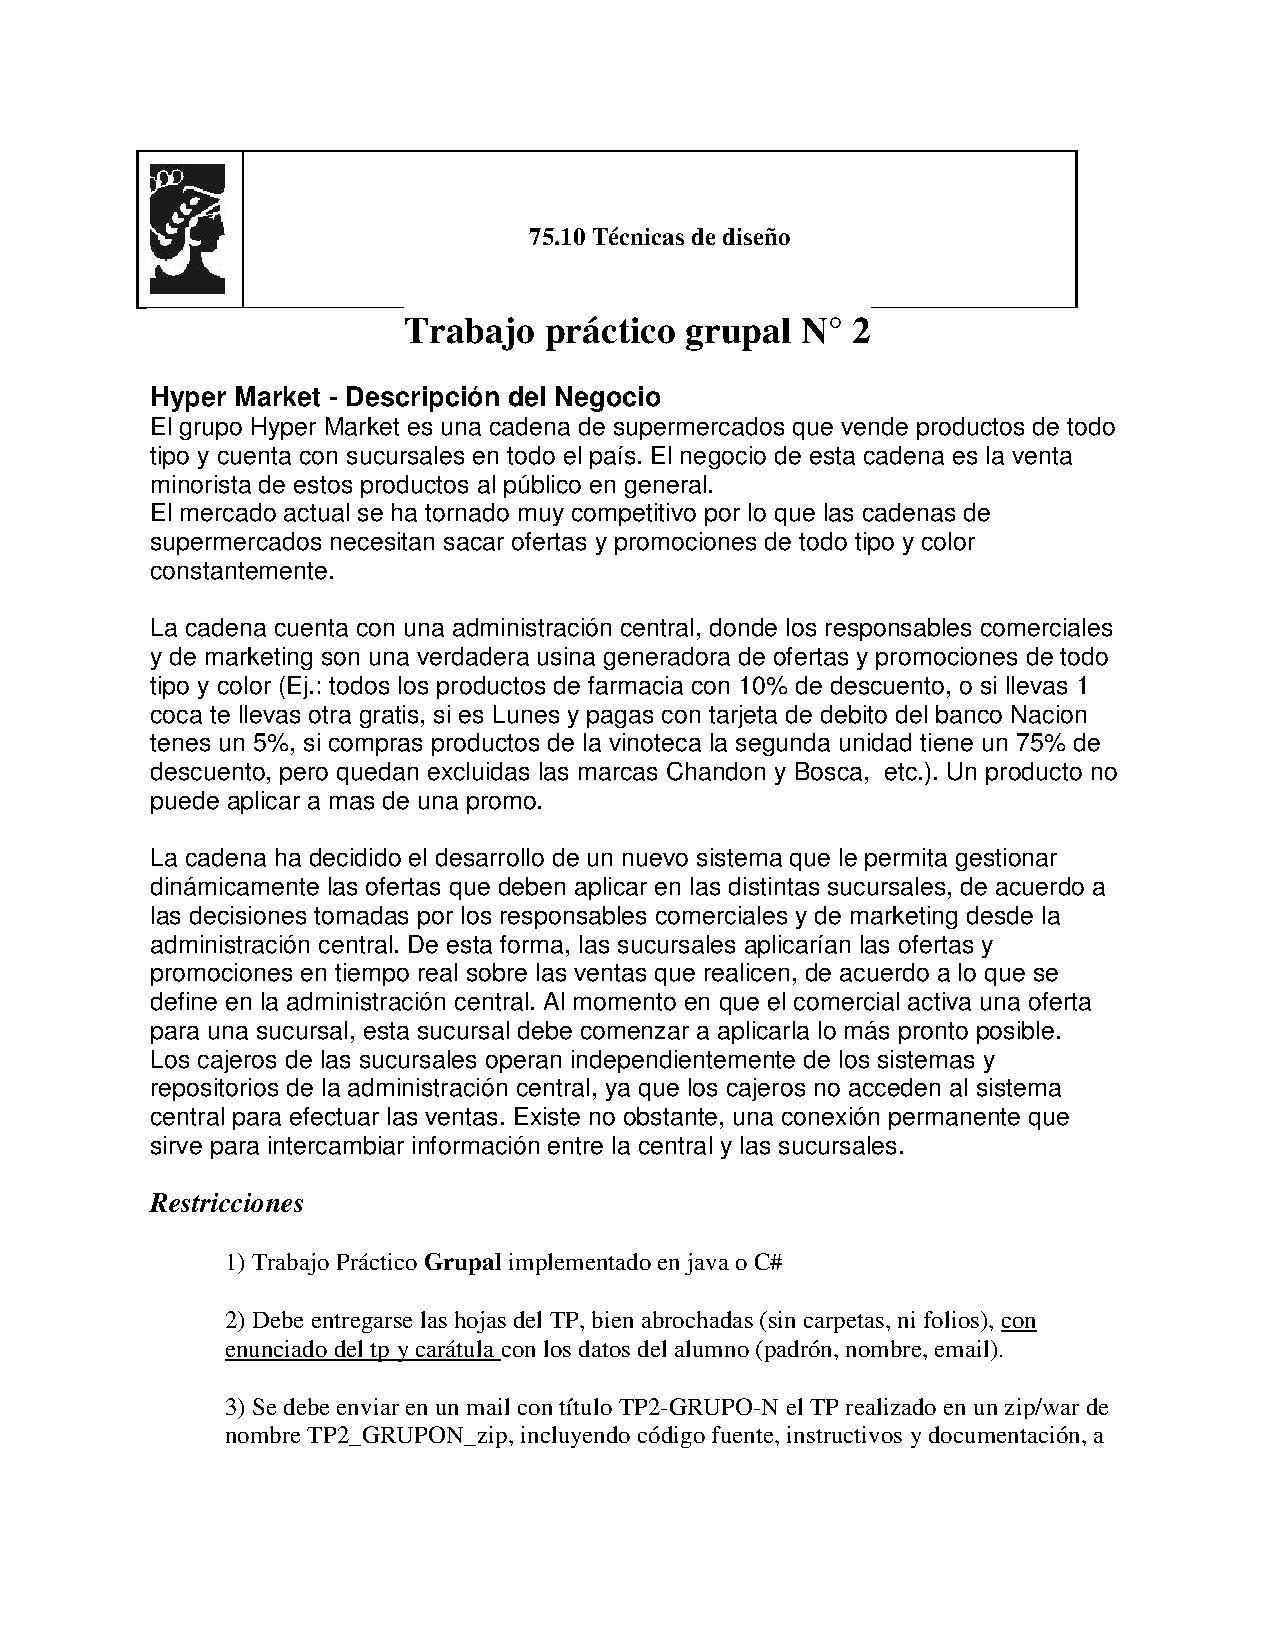
\includepdf[pages={-}, frame=true, pagecommand={}, noautoscale=true, scale=0.7]{src/docs/enunciado.pdf}

\end{document}

